\documentclass{article}
\usepackage{tikz}
\usetikzlibrary{arrows.meta}

\begin{document}

\begin{figure}[h]
    \centering
    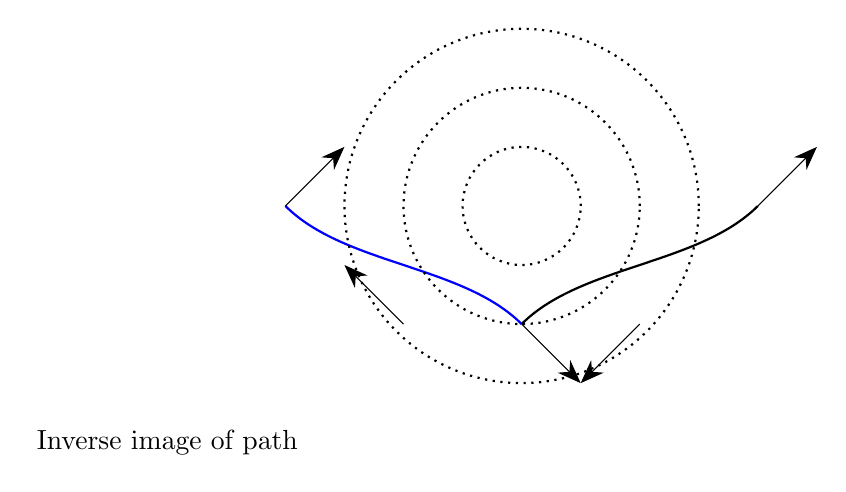
\begin{tikzpicture}[scale=1.5]
        % Define coordinates for the points
        \coordinate (A) at (-2,0);
        \coordinate (B) at (-1,-1);
        \coordinate (C) at (0,-1);
        \coordinate (D) at (1,-1);
        \coordinate (E) at (2,0);
        
        % Draw the path
        \draw[thick, blue] (A) .. controls (-1.5,-0.5) and (-0.5,-0.5) .. (C);
        \draw[thick, black] (C) .. controls (0.5,-0.5) and (1.5,-0.5) .. (E);
        
        % Draw the arrows
        \draw[-{Stealth[length=3mm]}] (A) -- ++(0.5,0.5);
        \draw[-{Stealth[length=3mm]}] (B) -- ++(-0.5,0.5);
        \draw[-{Stealth[length=3mm]}] (C) -- ++(0.5,-0.5);
        \draw[-{Stealth[length=3mm]}] (D) -- ++(-0.5,-0.5);
        \draw[-{Stealth[length=3mm]}] (E) -- ++(0.5,0.5);
        
        % Draw the dotted circles
        \draw[dotted, thick] (0,0) circle (1.5);
        \draw[dotted, thick] (0,0) circle (1);
        \draw[dotted, thick] (0,0) circle (0.5);
        
        % Label the image
        \node at (-3,-2) {Inverse image of path};
    \end{tikzpicture}
    \quad
    \begin{tikzpicture}[scale=1.5]
        % Define coordinates for the points
        \coordinate (A) at (0,0);
        \coordinate (B) at (1,0);
        \coordinate (C) at (2,0);
        \coordinate (D) at (3,0);
        
        % Draw the path
        \draw[thick, blue] (A) .. controls (0.5,1) and (1.5,1) .. (B);
        \draw[thick, blue] (B) .. controls (2.5,1) and (3.5,1) .. (C);
        \draw[thick, blue] (C) .. controls (4.5,1) and (5.5,1) .. (D);
        
        % Draw the arrows
        \draw[-{Stealth[length=3mm]}] (A) -- ++(0.5,0.5);
        \draw[-{Stealth[length=3mm]}] (B) -- ++(-0.5,0.5);
        \draw[-{Stealth[length=3mm]}] (C) -- ++(0.5,-0.5);
        \draw[-{Stealth[length=3mm]}] (D) -- ++(-0.5,-0.5);
        
        % Draw the dotted circles
        \draw[dotted, thick] (0,0) circle (1.5);
        \draw[dotted, thick] (0,0) circle (1);
        \draw[dotted, thick] (0,0) circle (0.5);
        
        % Label the image
        \node at (-3,-2) {Path associated to one Stokes arrow};
    \end{tikzpicture}
\end{figure}

\end{document}